\documentclass[12pt]{article}
\usepackage{graphicx}
\graphicspath{{assets/figures/}}
\usepackage{amsmath}
\usepackage[margin=1in]{geometry}
\usepackage{times}
\usepackage{caption}
\usepackage{hyperref}

\title{Chapter 3: Algorithmic Taint and the Machinery of Injustice}
\author{Ronald J. Botelho, MS}
\date{\today}

\begin{document}

\maketitle

\section*{Introduction}
Algorithmic tools are increasingly embedded in the scaffolding of governance, from surveillance to sentencing. While advertised as neutral, these systems frequently reproduce—and amplify—existing social biases.

\section*{The Invisible Hand of Code}
We begin by examining the ways that algorithms in public policy mimic corporate priorities, framing social services through a lens of efficiency rather than equity. These systems often obscure how decisions are made, shielding their logic behind proprietary code.

\begin{figure}[ht]
  \centering
  \includegraphics[width=0.9\textwidth]{algo_policy_footprint.png}
  \caption{Diffusion of algorithmic decision-making across state and federal services. Layman's explanation: What began as tech-sector optimization quietly became a governance model.}
\end{figure}

\section*{Feedback Loops of Harm}
Algorithmic decisions are not one-off events. They feed back into datasets, reinforcing prior judgments. This phenomenon, known as the feedback spiral, is especially dangerous in law enforcement and immigration systems, where flagged individuals are re-flagged based on prior alerts—many of which were generated by the algorithm itself.

\begin{figure}[ht]
  \centering
  \includegraphics[width=0.9\textwidth]{feedback_loop_model.png}
  \caption{Algorithmic feedback loop in risk scoring systems. Layman's explanation: The system learns from its own errors, then doubles down.}
\end{figure}

\section*{Black Boxes and Legal Gray Zones}
By outsourcing decisions to code, institutions have created legal ambiguity. Who is accountable when an algorithm discriminates? Corporations deny responsibility, citing the opacity of machine learning. Governments disclaim liability, claiming the systems are tested and fair. Victims are left with no human to challenge.

\section*{Conclusion: The Machinery of Injustice}
These systems are not neutral.\\
They are engineered.\\
And their effects are measurable—often at the expense of the most vulnerable.

This chapter concludes the first phase of our inquiry: institutional memory, privatized power, and algorithmic influence. What comes next is the democratic response.

\begin{figure}[ht]
  \centering
  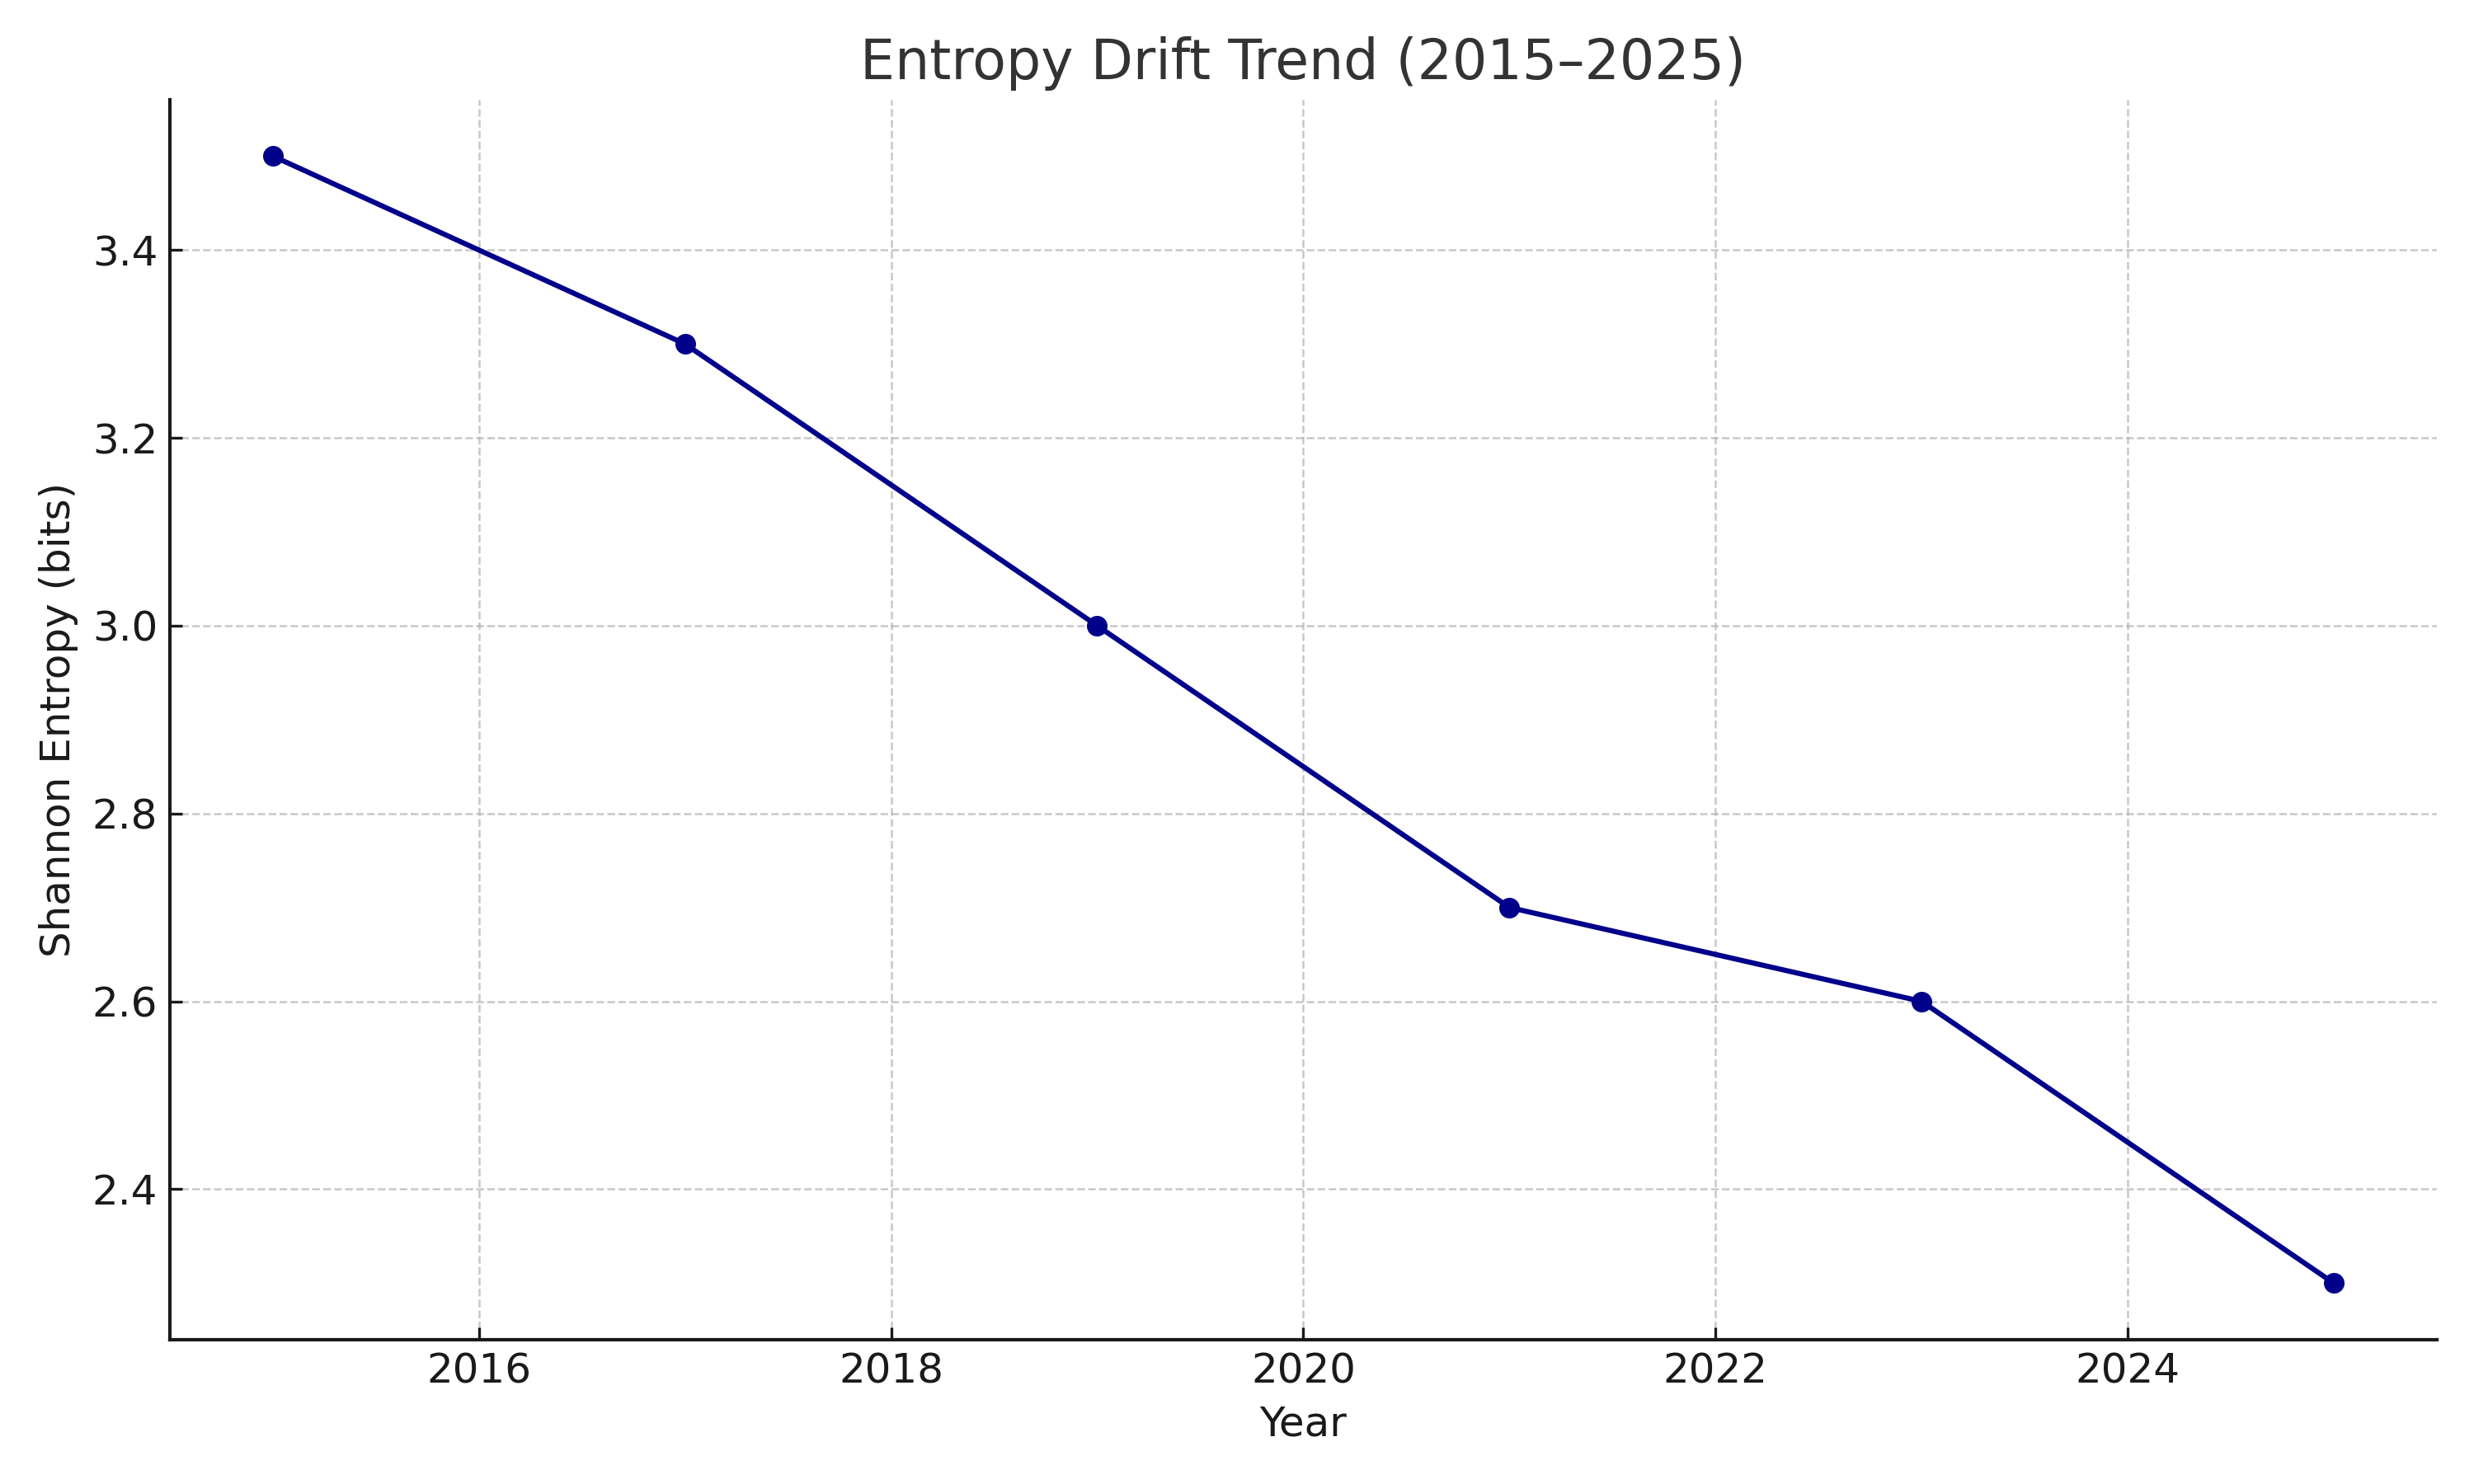
\includegraphics[width=0.9\textwidth]{entropy_drift_trend.png}
  \caption{Entropy drift trend in federal procurement data (source: FPDS-NG via Federal Compass).\\
  \textit{Layman's explanation:} Over time, the predictability—or disorder—of government procurement patterns shifts. These shifts reflect evolving priorities, policy shifts, or algorithmic optimization in contract awards. This plot shows how institutional decisions become increasingly machine-shaped.}
\end{figure}

\end{document}
